% Options for packages loaded elsewhere
% Options for packages loaded elsewhere
\PassOptionsToPackage{unicode}{hyperref}
\PassOptionsToPackage{hyphens}{url}
\PassOptionsToPackage{dvipsnames,svgnames,x11names}{xcolor}
%
\documentclass[
  number]{elsarticle}
\usepackage{xcolor}
\usepackage{amsmath,amssymb}
\setcounter{secnumdepth}{5}
\usepackage{iftex}
\ifPDFTeX
  \usepackage[T1]{fontenc}
  \usepackage[utf8]{inputenc}
  \usepackage{textcomp} % provide euro and other symbols
\else % if luatex or xetex
  \usepackage{unicode-math} % this also loads fontspec
  \defaultfontfeatures{Scale=MatchLowercase}
  \defaultfontfeatures[\rmfamily]{Ligatures=TeX,Scale=1}
\fi
\usepackage{lmodern}
\ifPDFTeX\else
  % xetex/luatex font selection
\fi
% Use upquote if available, for straight quotes in verbatim environments
\IfFileExists{upquote.sty}{\usepackage{upquote}}{}
\IfFileExists{microtype.sty}{% use microtype if available
  \usepackage[]{microtype}
  \UseMicrotypeSet[protrusion]{basicmath} % disable protrusion for tt fonts
}{}
\makeatletter
\@ifundefined{KOMAClassName}{% if non-KOMA class
  \IfFileExists{parskip.sty}{%
    \usepackage{parskip}
  }{% else
    \setlength{\parindent}{0pt}
    \setlength{\parskip}{6pt plus 2pt minus 1pt}}
}{% if KOMA class
  \KOMAoptions{parskip=half}}
\makeatother
% Make \paragraph and \subparagraph free-standing
\makeatletter
\ifx\paragraph\undefined\else
  \let\oldparagraph\paragraph
  \renewcommand{\paragraph}{
    \@ifstar
      \xxxParagraphStar
      \xxxParagraphNoStar
  }
  \newcommand{\xxxParagraphStar}[1]{\oldparagraph*{#1}\mbox{}}
  \newcommand{\xxxParagraphNoStar}[1]{\oldparagraph{#1}\mbox{}}
\fi
\ifx\subparagraph\undefined\else
  \let\oldsubparagraph\subparagraph
  \renewcommand{\subparagraph}{
    \@ifstar
      \xxxSubParagraphStar
      \xxxSubParagraphNoStar
  }
  \newcommand{\xxxSubParagraphStar}[1]{\oldsubparagraph*{#1}\mbox{}}
  \newcommand{\xxxSubParagraphNoStar}[1]{\oldsubparagraph{#1}\mbox{}}
\fi
\makeatother


\usepackage{longtable,booktabs,array}
\usepackage{calc} % for calculating minipage widths
% Correct order of tables after \paragraph or \subparagraph
\usepackage{etoolbox}
\makeatletter
\patchcmd\longtable{\par}{\if@noskipsec\mbox{}\fi\par}{}{}
\makeatother
% Allow footnotes in longtable head/foot
\IfFileExists{footnotehyper.sty}{\usepackage{footnotehyper}}{\usepackage{footnote}}
\makesavenoteenv{longtable}
\usepackage{graphicx}
\makeatletter
\newsavebox\pandoc@box
\newcommand*\pandocbounded[1]{% scales image to fit in text height/width
  \sbox\pandoc@box{#1}%
  \Gscale@div\@tempa{\textheight}{\dimexpr\ht\pandoc@box+\dp\pandoc@box\relax}%
  \Gscale@div\@tempb{\linewidth}{\wd\pandoc@box}%
  \ifdim\@tempb\p@<\@tempa\p@\let\@tempa\@tempb\fi% select the smaller of both
  \ifdim\@tempa\p@<\p@\scalebox{\@tempa}{\usebox\pandoc@box}%
  \else\usebox{\pandoc@box}%
  \fi%
}
% Set default figure placement to htbp
\def\fps@figure{htbp}
\makeatother





\setlength{\emergencystretch}{3em} % prevent overfull lines

\providecommand{\tightlist}{%
  \setlength{\itemsep}{0pt}\setlength{\parskip}{0pt}}



 
\usepackage[]{natbib}
\bibliographystyle{elsarticle-num}


\makeatletter
\@ifpackageloaded{caption}{}{\usepackage{caption}}
\AtBeginDocument{%
\ifdefined\contentsname
  \renewcommand*\contentsname{Table of contents}
\else
  \newcommand\contentsname{Table of contents}
\fi
\ifdefined\listfigurename
  \renewcommand*\listfigurename{List of Figures}
\else
  \newcommand\listfigurename{List of Figures}
\fi
\ifdefined\listtablename
  \renewcommand*\listtablename{List of Tables}
\else
  \newcommand\listtablename{List of Tables}
\fi
\ifdefined\figurename
  \renewcommand*\figurename{Figure}
\else
  \newcommand\figurename{Figure}
\fi
\ifdefined\tablename
  \renewcommand*\tablename{Table}
\else
  \newcommand\tablename{Table}
\fi
}
\@ifpackageloaded{float}{}{\usepackage{float}}
\floatstyle{ruled}
\@ifundefined{c@chapter}{\newfloat{codelisting}{h}{lop}}{\newfloat{codelisting}{h}{lop}[chapter]}
\floatname{codelisting}{Listing}
\newcommand*\listoflistings{\listof{codelisting}{List of Listings}}
\captionsetup{labelsep=period}
\makeatother
\makeatletter
\makeatother
\makeatletter
\@ifpackageloaded{caption}{}{\usepackage{caption}}
\@ifpackageloaded{subcaption}{}{\usepackage{subcaption}}
\makeatother
\usepackage{bookmark}
\IfFileExists{xurl.sty}{\usepackage{xurl}}{} % add URL line breaks if available
\urlstyle{same}
\hypersetup{
  pdftitle={The R \textgreater{} E Phenomenon and the Distance-Difficulty Hypothesis: Modeling Response Time in Attitudinal Data},
  pdfauthor={Nicole G. Bonge; Ronna C. Turner},
  pdfkeywords={Response Time, Item Response Theory, Distance-Difficulty
Hypothesis, F \textgreater{} C Phenomenon},
  colorlinks=true,
  linkcolor={blue},
  filecolor={Maroon},
  citecolor={Blue},
  urlcolor={Blue},
  pdfcreator={LaTeX via pandoc}}


\setlength{\parindent}{6pt}
\begin{document}

\begin{frontmatter}
\title{The R \textgreater{} E Phenomenon and the Distance-Difficulty
Hypothesis: Modeling Response Time in Attitudinal Data}
\author[1]{Nicole G. Bonge%
%
}
 \ead{ngbonge@uark.edu} 
\author[1]{Ronna C. Turner%
\corref{cor1}%
}
 \ead{rcturner@uark.edu} 

\affiliation[1]{organization={University of Arkansas},,postcodesep={}}

\cortext[cor1]{Corresponding author}


        
\begin{abstract}
Response time (or response latency) is a commonly used metric to assess
item characteristics such as quality or comprehensibility, and
respondent characteristics such as fatigue or effort. In this study, we
apply response time models to attitudinal data, showing that survey item
response time is related to a respondent's latent trait level and item
difficulty in relation to the respondent's latent trait level
(distance-difficulty hypothesis). We also investigate the R
\textgreater{} E phenomenon, demonstrating that respondents take longer
to refute items than to endorse them. Our results indicate that response
time involves complex cognitive processes, and we caution researchers
against using response time as a metric when assessing item or
respondent characteristics (such as respondent effort or item quality)
without controlling for other factors such as trait level,
distance-difficulty item-person relationships, and item agreement. It is
recommended that researchers conducting data quality assessments
evaluate the occurrence of low data quality flagging for participants at
different construct levels, to determine whether overidentification of
participants in certain ability ranges may be related to item difficulty
location.
\end{abstract}





\begin{keyword}
    Response Time \sep Item Response Theory \sep Distance-Difficulty
Hypothesis \sep 
    F \textgreater{} C Phenomenon
\end{keyword}
\end{frontmatter}
    

\section{Introduction}\label{introduction}

As computerized psychological testing has gained popularity over the
past several decades, researchers are able to collect response time
information alongside item responses at minimal~cost. It is a widely
held belief among survey researchers that response time is indicative of
the cognitive effort required to answer an item (Höhne et al., 2017);
thus, researchers point to response time to assess item quality and
comprehensibility (Bassili et al., 1996; Lenzner, 2012; Lenzner et al.,
2010). Researchers have also used response time to detect respondent
fatigue (Nguyen, 2017), insufficient effort responding (Bowling et al.,
2023; Krosnick, 1991; Ulitzsch et al., 2022), and other aberrant
response patterns (van der Linden \& van Krimpen-Stoop, 2003).
Researchers have also used response time to investigate cognitive
processes underlying item responses (De Boeck \& Jeon, 2019).

In this study, we extend a set of models proposed by Tancoš et
al.~(2023) ~to attitudinal data and investigate how response time
relates to several factors, including item difficulty, the strength of
the latent trait of the respondent, and whether the respondent endorses
the behavior described in the survey item. The models include an
assessment of the distance-difficulty hypothesis (Lorenzo-Seva, 2007a;
Thissen, 1983), which states that response time increases with
decreasing person-item distance (that is, the distance between the
respondent's trait level and the item's neutral threshold on the latent
trait continuum). Moreover, we introduce the R \textgreater{} E
phenomenon, an attitudinal analog to the ``F \textgreater{} C
phenomenon'' seen in achievement contexts (Beckmann, 2000), where
respondents take longer to provide incorrect answers than correct ones.
The R \textgreater{} E phenomenon reflects our observation that
respondents take longer to disagree with an attitudinal item than to
agree with it. Finally, we investigate an interaction effect between the
distance-difficulty hypothesis and the R \textgreater{} E phenomenon.
Our study is designed to add to the body of literature regarding the
complex processes involved in item responses and provides information
about the use of response time when measuring item quality or respondent
effort.

\section{Theoretical Framework}\label{theoretical-framework}

\subsection{The F \textgreater{} C Phenomenon}\label{the-f-c-phenomenon}

In the context of achievement testing, the F \textgreater{} C phenomenon
(Beckmann, 2000), also called the I \textgreater{} C phenomenon, posits
that false responses take longer to report than correct ones. Formally
the F \textgreater{} C phenomenon is given by(Beckmann, 2000, as cited
in Tancoš et al., 2023, p.~3):

\[
t_{ij} = \mu + \gamma FC_{ij}+\epsilon_{ij},
\]

where \(t_{ij}\) is the response time of person \(j\) on item \(i\);
\(\mu\) is an intercept which describes the average time across each
item and person; \(FC_{ij}\) is a binary indicator of whether person
\(j\) answered item \(i\) correctly; \(\gamma\) is an unstandardized
regression coefficient describing the mean difference in response time
between false and correct answers; and \(\epsilon_{ij}\) is a normally
distributed residual. The F \textgreater{} C phenomenon has been
demonstrated to be a significant predictor of response time in a number
of prior studies for cognitive and achievement testing (e.g., Goldhammer
et al., 2014; Goldhammer et al., 2015; Lasry et al., 2013; Preckel \&
Freund, 2005).

\subsection{The Distance-Difficulty
Hypothesis}\label{the-distance-difficulty-hypothesis}

Originally proposed by Thissen (1983) and later revised by Ferrando and
Lorenzo-Seva (2007a), the distance difficulty hypothesis states that the
response time for an item decreases as the distance between the
respondent's ability, or trait, level (\(\theta_j\)) and the item
difficulty (\(b_i\)), given by \(\delta_{ij}=|θ_j-b_i|\) increases. That
is, a respondent should take more time to answer a question that is
close to their trait level. On the other hand, a respondent should take
less time to answer a question that is very easy or very difficult
relative to their trait level. Thissen's model (1983, p.~181) is given
by: \[ \log{(t_{ij})} = \nu + s_i+u_j - bz_{ij}+\epsilon_{ij},\] where
\(\log{(t_{ij})}\) is a logarithmic transformation of the response time
for person \(j\) on item \(i\) (this transformation is meant to achieve
normally distributed errors \(\epsilon_{ij}\)); \(\nu\) is the
intercept, representing the overall mean log response time; \(s_i\)
describes the average time respondent \(i\) spent across all items;
\(u_j\) is the time required by a person of average ability to answer
item \(j\); and \(b\) is the regression coefficient representing the
relationship of response latency with respondent ability and item
easiness (in \(z_{ij}=a_j θ_i+c_j\), where \(a_j\) is the discrimination
of item \(j\), \(c_j\) is the easiness of item \(j\), and \(θ_i\) is the
ability level of respondent \(i\)). Ferrando and Lorenzo-Seva (2007a,
p.~528) proposed the following as an alternative person-item distance
measure according to the two-parameter logistic (2PL) model:
\[\delta_{ij}=\sqrt{a_i^2 (θ_j-b_i )^2},\] where \(a_i\) is
discrimination for item \(i\). In well-designed items, \(a_i\) is
positive, and in this case, we can simplify the term to
\(\delta_{ij}=a_i|θ_j-b_i|\).

Heretofore, the models describing the distance-difficulty hypothesis
have been designed for use with binary data. Ferrando and Lorenzo-Seva
(2007b, p.~679) extended the distance-difficulty hypothesis to a model
intended for use with graded or continuous items measuring a
unidimensional construct, where the person-item distance is given by:
\[\delta_{ij}=\sqrt{(θ_i-τ_j)^2},\] where \(\tau_j\) is the ``item
threshold,'' the point on the trait continuum, marking the point at
which respondents are more likely to agree with an item than disagree
with it. The distance-difficulty hypothesis was originally used with
spatial ability (Thissen, 1983) but has also been extended to
personality scales (e.g., Ferrando, 2006).

\subsection{The Tancoš Models}\label{the-tancoux161-models}

Tancoš et al.~(2023) proposed two sets of models relating to fluid
intelligence in children: first, a model focused on the F \textgreater{}
C phenomenon, which controls for item difficulty (\(b_i\)) and
respondent ability (\(\theta_j\)) with an added interaction term of
answer correctness (\(FC_{ij}\)) and respondent ability. This model is
given by (Tancoš et al., 2023, p.~7):
\[\ln{(t_{ij})}=\mu+\nu_j+\beta_i+\gamma_1 FC_{ij}+\gamma_2 b_i+\gamma_3 \theta_j+\gamma_{13} FC_{ij}\theta_j+\epsilon_{ij},\]
where \(\ln{t_{ij}}\) is a logarithmic transformation of the response
time for person \(j\) on item \(i\); \(\mu\) is the fixed intercept
(representing the time spent by an average-ability respondent on an
average-difficulty item); \(\nu_j\) is the random intercept for each
person (general speediness of respondent \(j\); the average time
respondent \(j\) spent across all items); \(\beta_i\) is the random
intercept for each item (time required by a person of average ability to
answer item \(i\)); \(\gamma_1\), \(\gamma_2\), \(\gamma_3\), and
\(\gamma_{13}\) are the fixed effects of the corresponding predictors;
and \(\epsilon_{ij}\) is the normally distributed residual.

The second model Tancoš et al.~(2023) proposed assesses the
distance-difficulty hypothesis and investigates its incremental validity
over the F \textgreater{} C phenomenon. This model is represented by
(Tancoš et al., 2023, p.~8):
\[\ln{(t_{ij})}=\mu+\nu_j+\beta_i+\gamma_4 \delta_{ij}+\gamma_1 FC_{ij}+\gamma_{14} FC_{ij} \delta_{ij}+\epsilon_{ij},\]
where \(\ln{(t_{ij})}\) is a logarithmic transformation of the response
time for person \(j\) on item \(i\); \(\mu\) is the fixed intercept;
\(\nu_j\) is the random intercept for each person; \(\beta_i\) is the
random intercept for each item; \(\delta_{ij}=|\theta_j-b_i|\) is the
absolute distance between respondent \(j\)'s ability level and item
\(i\)'s difficulty; \(FC_{ij}\) is a binary variable representing item
correctness; \(\gamma_1\), \(\gamma_2\), \(\gamma_3\), and
\(\gamma_{13}\) are the fixed effects of the corresponding predictors;
and \(\epsilon_{ij}\) is the normally distributed residual.

In their study, Tancoš et al.~(2023) found that the F \textgreater{} C
phenomenon remained significant after controlling for item difficulty
and person ability, with an interaction between ability level and
response correctness. Furthermore, ability level impacted response time
(though only in items with moderate or high difficulty), but item
difficulty did not influence response time. Taken together, the results
indicated that on items with moderate-to-high difficulty, children with
higher ability levels took longer to report incorrect answers than
children with lower ability levels. However, Tancoš et al.~(2023) found
no relationship between ability level and response time with correct
answers, challenging the `faster equals smarter' stereotype.

Moreover, Tancoš et al.~(2023) found incremental validity of the
distance-difficulty hypothesis above and beyond the F \textgreater{} C
phenomenon, providing support for the distance-difficulty hypothesis and
its interaction with the F \textgreater{} C phenomenon. These results
imply items that match a respondent's ability level take the longest to
answer, with increased time required for incorrectly answered items.
Furthermore, as \(\delta_{ij}\) increased, they found that the
difference in response time narrows and eventually changes direction.
That is, when an item is very easy or very difficult in relation to a
respondent's ability level, respondents take longer to report correct
answers than false ones.

\section{The Proposed Models}\label{the-proposed-models}

In this study, we adapt the Tancoš models to personality testing, using
answer endorsement instead of answer correctness as an interaction term.
Specifically, we test an attitudinal analog of the F \textgreater{} C
phenomenon, postulating it takes respondents more time to refute, or
disagree with, an item than endorse, or agree with, it. We call this
version of the F \textgreater{} C phenomenon the `R \textgreater{} E
phenomenon.' This hypothesis is related to prior research on the F
\textgreater{} C phenomenon (citation), and neuroscience research
related to brain functioning during in-person interactions of agreement
versus disagreement. For example, Hirsch et al.~(2021) found that brain
activity differed during interactions that included attitudinal
agreement vs disagreement with lower levels of synchronous dyadic brain
functioning during disagreement, potentially related to more complex
cognitive load. If the R \textgreater{} E phenomenon holds, we will then
investigate whether there is a significant interaction between the R
\textgreater{} E phenomenon and the ability-difficulty distance (using
an item's neutral threshold in place of item difficulty as described by
Ferrando and Lorenzo-Seva (2007a), since our data are polytomous and not
binary). Such an interaction would suggest that there is a difference in
the relationship between the time needed to respond to an item and the
ability-difficulty distance among respondents who endorse the item and
those who refute it.

\section{Method}\label{method}

\subsection{Participants and Measures}\label{participants-and-measures}

We examined data from the free online Machiavellianism scale (MACH-IV),
developed by Christie and Geis (1970), from
https://openpsychometrics.org/tests/MACH-IV. Before beginning the test,
respondents agreed that their anonymous data could be used for research.
Following the 20-item test, respondents were prompted with a 13-item
survey containing general demographic questions. Each test question and
survey question was presented on separate pages, with response time
recorded as the amount of time, in milliseconds, spent per page. See
Appendix 1 for MACH-IV item prompts.

Prior to testing the research questions, we conducted data quality
analyses to select data that are less likely to be impacted by random or
careless responding, which can decrease the accuracy of results (e.g.,
DeSimone \& Harms, 2017; Huang et al., 2012). The dataset contained a
vocabulary check as a direct data quality assessment in which
respondents were prompted to indicate the words from a list of 16, of
which they were sure they knew the definition. Three of the words were
not real, so we removed responses where those words were selected. We
also set aside respondents whose total test or survey time fell in the
bottom or top decile, as an indirect data quality assessment. Our
rationale for this choice is that respondents who fell in the bottom
decile may not have spent sufficient time on the questions to provide
reliable results (e.g., Reimers et al., 2023); whereas, respondents in
the top decile of response time may not have completed the scale in a
single sitting or without distraction. Third, we used the careless
package in R (v1.2.2; Yentes \& Wilhelm, 2023) to quantify longstring
responses, the length of the maximum uninterrupted string of identical
responses. We elected to remove responses with five or more identical
consecutive responses, corresponding to the 95th percentile from this
sample. Note, half of the items were reverse worded, with alternating
placement used (see Appendix 1). For reference, the mean and median
number of identical successive responses were 2.93 and 3.0,
respectively.

Our final sample consisted of 11,772 adults, 48.9\% female, who
completed the scale in the United States and reported English was their
native language. Only complete responses were considered. The average
respondent age was 35.2 years, with reported ages ranging from 18 to 91
years.

\subsection{Initial IRT Analysis}\label{initial-irt-analysis}

All analyses were conducted using R Statistical Software (v4.3.2; R Core
Team, 2023). We began by performing an exploratory factor analysis (EFA)
using the psych package in R (v2.4.3; Revelle, 2024) with all twenty
items from the MACH-IV scale, reverse-coding negatively worded items
before analysis. As the purpose of this study was to test the effects of
question location (difficulty) and latent ability on response time and
not on the interpretation of people's level of Machiavellianism, we
choose to set aside items that did not fit a one-factor model well. We
did not want the results impacted by items measuring secondary nuisance
factors rather than the variables being investigated. One item had
insufficient factor loading (\textless{} .40). This item was set aside
form the original 20, and we performed another EFA; an unweighted least
squares estimation yielded sufficient factor loadings for a one-factor
model. Given these results, we performed a unidimensional item response
theory (IRT) analysis using the mirt R package (v1.41; Chalmers, 2012).
Beginning with a comparison between the graded response model (GRM) and
the generalized partial credit model (GPCM), model fit indices (AIC,
BIC, SABIC, and log-likelihood) indicated that the GRM fit better than
the GPCM (Table~\ref{tbl-Table1}).

We proceeded with the GRM, extracting each item's neutral threshold
(\(\tau_{i,N}\); the point on the latent trait continuum at which
respondents are more likely to ``agree'' or ``strongly agree'' with an
item than to be ``neutral,'' ``disagree,'' or ``strongly disagree'' with
the item), discrimination (\(a_i\)), and each respondent's estimated
ability parameter (\(\theta_j\)). See Table~\ref{tbl-Table2} for item
descriptive statistics and GRM parameters. Empirical reliability was
high (\(r_{\text{coefficient alpha}} = .91\)).

\subsection{Main Analysis}\label{main-analysis}

Our main analysis involved two sets of nested linear multilevel
regression models. The first set of models tested the R \textgreater{} E
phenomenon, controlling for item difficulty and respondent ability; the
second set of models tested the distance-difficulty hypothesis and its
interaction with the R \textgreater{} E phenomenon. We used the lme4
package (v1.1-35.3; Bates et al., 2015) to estimate each model, and
after estimating, we computed the variance inflation factor (VIF) using
the car package (v3.1-2; Fox \& Weisberg, 2019) to check for
multicollinearity. Finally, we used the lmerTest package (v3.1-3;
Kuznetsova et al., 2017) to compare models.

First, we estimated a null model (Model 0) as a baseline for both sets
of models. Consistent with Tancoš et al.~(2023), Model 0 only included
fixed and random intercept terms for respondents and items; all models
used logarithmic transformation of response time for the dependent
variable to linearize the relationship between the predictor variables
and response time. We then defined the first series of models: Model A1
includes only a binary predictor for endorsement (\(E_{ij}\)); Model A2
includes two predictors, item neutral threshold (\(\tau_{i,N}\)) and
respondent ability (\(\theta_j\)), as control variables; Model 3
includes the interaction term of answer endorsement and respondent
ability to investigate the impact of respondent ability on the R
\textgreater{} E phenomenon. Model A3 is as follows:

\[\ln{(t_{ij})}=\mu + \nu_j +\beta_i+\gamma_1E_{ij}+\gamma_2\tau_{i,N}+\gamma_3\theta_j +\gamma_{13}E_{ij}\theta_j+\epsilon_{ij},\]
where \(E_{ij}\), \(\tau_{i,N}\), and \(\theta_j\) are defined above;
\(\mu\) is the fixed intercept representing the time spent by an
average-ability respondent on an average-difficulty item; \(\nu_j\) is
the random intercept for each person (general speediness of respondent
j; the average time respondent j spent across all items); \(\beta_j\) is
the random intercept for each item (time required by a person of average
ability to answer item i); \(\gamma_1\), \(\gamma_2\), \(\gamma_3\), and
\(\gamma_{13}\) are the fixed effects of the corresponding predictors;
and \(\epsilon_{ij}\) is the normally distributed residual. See Appendix
2 for a complete list of models tested.

The second set of models began with Model B1, testing the
distance-difficulty hypothesis by including only the
discrimination-adjusted absolute difference between the respondent
ability and the neutral threshold for each item
(\(\delta_{ij}=a_i |θ_j-τ_{i,N} |\)). Model B2 incorporates \(E_{ij}\),
a binary variable to represent the R \textgreater{} E phenomenon, to
assess the incremental validity of the R \textgreater{} E phenomenon
beyond the distance-difficulty hypothesis. Finally, Model B3 includes
the interaction term of the distance \(\delta_{ij}\) with answer
endorsement (\(E_{ij}\)), to investigate whether the distance-difficulty
effect follows a different pattern when respondents endorse an item or
refute it. Model B3 is given by:
\[\ln{(t_{ij})}=\mu+\nu_j+\beta_i+\gamma_4 \delta_{ij}+\gamma_1 E_{ij}+\gamma_{14} E_{ij}\delta_{ij}+\epsilon_{ij},\]
where all variables are defined as stated above.

\section{Results}\label{results}

\subsection{Null Model}\label{null-model}

The null model, Model 0, provided a baseline for each set of models .
The fixed intercept was significant (\(μ=8.87\), 95\% CI {[}8.73,
9.00{]}) and can be interpreted as the average response time of a
respondent who is of average-ability on an average-difficulty item.
Transforming the parameter from its logarithmic form and converting from
milliseconds to seconds, we see the average response time was 7.12
seconds. Table~\ref{tbl-Model0} displays complete results for Model 0.

\subsection{Models Assessing the R \textgreater{} E
Phenomenon}\label{models-assessing-the-r-e-phenomenon}

Beginning with Model A1, we found it took respondents significantly
longer to endorse an item than to refute it (\(γ_1=-0.07\), 95\% CI
{[}-0.07, -0.06{]}) The effect size is small, however, with the
transformed parameter of 0.48 seconds, signifying the expected average
difference in response time between endorsement and rejections.
Table~\ref{tbl-ModelA1} displays complete results for Model A1.

In Model A2, the R \textgreater{} E phenomenon remained significant
after controlling for item difficulty and respondent trait level
(\(γ_1=-0.04\), 95\% CI {[}-0.04, -0.03{]}). Moreover, we found that
respondents with higher levels of Machiavellianism took significantly
less time to respond to questions than respondents with lower levels
(\(γ_3=-0.04\), 95\% CI {[}-0.05, -0.04{]}). Moreover, response time was
significantly related to the location of the item's neutral threshold
(\(γ_2=0.19\), 95\% CI {[}0.03, 0.35{]}). Table~\ref{tbl-ModelA2}
displays complete results for Model A2.

In Model A3, the added interaction between endorsement and trait level
was not significant (\(γ_{13}=0.00\), 95\% CI {[}-0.01,0.00{]}).
Table~\ref{tbl-ModelA3} displays complete results for Model A3.
Moreover, per the information criteria and goodness-of-fit measures,
Model A3 did not fit the data better than the preceding model in the
series (Table~\ref{tbl-Series1}). Thus, we retain Model A2 as this
series' final model.

All effects combined, Model A2 indicates that respondents took
significantly longer to refute items than to endorse them, regardless of
trait level or the item's neutral threshold. Further, respondents took
longer to answer items with higher neutral thresholds, but response time
decreased with increasing trait level, holding all other variables
constant. Figure~\ref{fig-Figure1} reflects this pattern.

\subsection{Models Assessing the Distance-Difficulty
Hypothesis}\label{models-assessing-the-distance-difficulty-hypothesis}

In Model B1, we investigated the logarithm-transform of response time as
a function of the ability-difficulty distance. The effect of the
ability-difficulty distance was significant (\(γ_4=-0.07\), 95\% CI
{[}-0.07, -0.06{]}). From this, we see the response time decreased by
6.8\% with each logit unit increase of ability-difficulty distance. For
example, the average response time was 7.71 seconds for respondents
whose trait level matched the item's neutral threshold (i.e., the
discrimination-adjusted ability-difficulty difference was zero);
response time decreases to 7.19 seconds when the ability-difficulty
distance is one logit unit, and 6.70 seconds when the distance is two
logit units. Table~\ref{tbl-ModelB1} displays complete results for Model
B1.

In Model B2, we added an Endorsement fixed effect, which was significant
(\(γ_1=-0.04\), 95\% CI {[}-0.04, -0.03{]}), indicating endorsement
resulted in a significantly shorter response time than non-endorsement.
The ability-difficulty distance effect was not substantially affected by
the additional predictor (\(γ_4=-0.06\), 95\% CI {[}-0.07, -0.06{]}).
Table~\ref{tbl-ModelB2} displays complete results for Model B2.

Model B3 extended Model B2 by adding the interaction of the
ability-difficulty distance effect and the Endorsement effect, which was
significant (\(γ_{14}=-0.01\), 95\% CI {[}-0.01,0.00{]}). We see a
reduced, but still significant, effect in Endorsement (\(γ_1=-0.03\),
95\% CI {[}-0.052,-0.037{]}) while the estimated ability-difficulty
distance effect (\(γ_4=-0.06\), 95\% CI {[}-0.06,-0.06{]}) remained the
same. Complete results for Model B3 are shown in
Table~\ref{tbl-ModelB3}.

Overall, each model fit significantly better than the preceding model in
the series according to model fit and information criteria
(Table~\ref{tbl-Series2}). Model B3 fit the data significantly better
than the preceding model according to the goodness-of-fit test, AIC, and
log-likelihood value. Thus, we retained Model B3 as our final model.
These estimates indicate that response times were significantly lower
for people whose trait was significantly farther away from the item
difficulty as compared to those who trait was close to the item
difficulty level, with longer times overall for respondents who rejected
the item in comparison to those who endorsed the item. Although the
differences were small, the impact of rejecting versus endorsing an item
were larger when the item difficulty was further away from the person's
trait level. Figure~\ref{fig-Figure2} displays this pattern.

\section{Discussion}\label{discussion}

This study introduces the R \textgreater{} E Phenomenon, an attitudinal
extension of the F \textgreater{} C phenomenon seen in achievement
settings. In particular, we followed the Tancoš et al.~(2023)
methodology by investigating two phenomena: first, we assessed whether
the R \textgreater{} E phenomenon was a significant predictor of
response time after controlling for participants' trait levels and item
difficulties (operationalized in this context as an item's neutral
threshold). Our data show that, after controlling for trait level and
item difficulty, respondents took longer to refute items than to endorse
them. While the effect size is small, the R \textgreater{} E phenomenon
accounts for significant variability in response time.

These findings may have multiple causes. Kowalski et al.~(2018) found
Machiavellianism is positively predicted by fluid intelligence, ``the
ability to be flexible and to respond adaptively to novel situations''
(Gilhooly \& Gilhooly, 2021, p.~186). A respondent with greater fluid
intelligence may be able to assess whether, and how, an item applies to
their life faster than someone with a lower level of fluid intelligence.
Another explanation for the observed differences in response time
between endorsing and rejecting an item could be that respondents who
agree with an item can more quickly articulate applications of the item
to their own lives. In contrast, respondents who do not endorse an item
may think through a variety of situations in which the item may apply
but ultimately does not. These results may also correspond with
neuroscience research (e.g., Hirsch et al., 2021) that brain functioning
for interactions related to agreement may be less complex than what is
used for interactions where one disagrees.

Since the R \textgreater{} E phenomenon held after controlling for
participant trait level and item difficulty, we investigated the
distance-difficulty hypothesis and its interaction with the R
\textgreater{} E phenomenon. We found evidence to support the
distance-difficulty hypothesis in the context of an attitudinal survey,
and a significant interaction between the distance-difficulty hypothesis
and the R \textgreater{} E phenomenon. The most substantial impact was
the decrease in response time with increasing distance between the
respondent's trait level and the item's neutral threshold (that is,
respondents answered faster to questions they more strongly agreed or
disagreed with) and overall, the time used to answer the questions was
consistently longer for those rejecting the questions rather than
endorsing.

Response time is a metric often used to assess participants' response
effort and item characteristics including difficulty, exposure,
interpretability, and suitability. Given the results of this study, we
caution researchers against using response time alone to make such
determinations. This study adds to the body of knowledge regarding the
complexity of item response processes and challenges the practice of
using response time in isolation to make determinations about respondent
effort or item complexity and suitability.

\section*{References}\label{references}
\addcontentsline{toc}{section}{References}

\renewcommand{\bibsection}{}
\bibliography{references.bib}

\section*{Tables}\label{tables}
\addcontentsline{toc}{section}{Tables}

\begin{longtable}[]{@{}lllll@{}}

\caption{\label{tbl-Table1}IRT Model Comparison}

\tabularnewline

\toprule\noalign{}
Model & AIC & BIC & SABIC & Log-Likelihood \\
\midrule\noalign{}
\endhead
\bottomrule\noalign{}
\endlastfoot
GRM & 579,083.8 & 579,780.8 & 579,478.9 & -289,446.9 \\
GPCM & 583,294.6 & 583,991.5 & 583,689.6 & -291,552.3 \\

\end{longtable}

\begin{longtable}[]{@{}lllllll@{}}

\caption{\label{tbl-Table2}Descriptive Statistics for Items}

\tabularnewline

\toprule\noalign{}
& & & \multicolumn{2}{l}{%
Response} & \multicolumn{2}{l@{}}{%
Response Time (milliseconds)} \\
Item & Item Neutral Threshold & Item Discrimination & M & SD & M & SD \\
\midrule\noalign{}
\endhead
\bottomrule\noalign{}
\endlastfoot
1 & 0.30 & 1.94 & 2.87 & 1.52 & 9,291.49 & 8,165.46 \\
2 & 0.22 & 1.62 & 2.88 & 1.46 & 7,775.72 & 6,310.25 \\
3R & 0.22 & 1.05 & 3.10 & 1.41 & 10,281.67 & 8,464.00 \\
4R & 0.50 & 1.34 & 2.93 & 1.38 & 5,936.70 & 5,586.97 \\
5 & -0.18 & 1.52 & 3.29 & 1.41 & 10,830.67 & 8,278.18 \\
6R & -0.07 & 1.62 & 3.25 & 1.48 & 5,399.48 & 5,327.17 \\
7R & -0.81 & 1.54 & 3.78 & 1.35 & 6,282.45 & 5,411.08 \\
8 & 0.36 & 1.33 & 2.80 & 1.46 & 8,434.98 & 6,999.64 \\
9R & 1.43 & 2.03 & 1.86 & 1.20 & 9,972.70 & 7,810.57 \\
10R & 0.51 & 1.69 & 2.67 & 1.45 & 15,841.10 & 11,889.62 \\
11R & -1.56 & 1.05 & 4.20 & 1.04 & 7,746.36 & 5,758.39 \\
12 & -0.45 & 1.50 & 3.49 & 1.46 & 7,939.62 & 6,740.82 \\
13 & 0.43 & 1.54 & 2.68 & 1.53 & 10,911.95 & 8,602.82 \\
14R & -0.63 & 1.22 & 3.76 & 1.20 & 5,143.86 & 4,445.55 \\
15 & -0.18 & 1.29 & 3.32 & 1.38 & 6,622.52 & 5,061.89 \\
16R & -0.29 & 1.03 & 3.36 & 1.51 & 6,896.94 & 5,771.57 \\
17R & -0.89 & 0.94 & 3.80 & 1.32 & 9,319.10 & 6,862.45 \\
18 & -0.21 & 1.47 & 3.27 & 1.42 & 7,883.50 & 6,581.88 \\
20 & 1.73 & 0.97 & 2.04 & 1.36 & 12,581.28 & 8,816.57 \\

\end{longtable}

\emph{Note.} Items ending in ``R'' were reverse coded before statistical
analysis.

\begin{longtable}[]{@{}llllll@{}}

\caption{\label{tbl-Model0}Parameters for Model 0}

\tabularnewline

\toprule\noalign{}
& & & & \multicolumn{2}{c@{}}{%
95\% CI} \\
& Coef. & Est. & & LL & UL \\
\midrule\noalign{}
\endhead
\bottomrule\noalign{}
\endlastfoot
\emph{Fixed Effects} & & & & & \\
Intercept & μ & 8.87 & *** & 8.73 & 9.00 \\
\emph{Random Effects} & & & & & \\
Person intercept variance & var(\emph{ν\textsubscript{j}} ) & 0.05 & ***
& & \\
Item intercept variance & var(\emph{β\textsubscript{i}} ) & 0.09 & *** &
& \\
Residual Variance & var(\emph{ε\textsubscript{ij}} ) & 0.24 & & & \\

\end{longtable}

\emph{Note.} Coef -- coefficient; Est -- estimate; CI -- confidence
interval; LL -- lower limit; UL -- upper limit; Var -- variance. * p
\textless{} .05, ** p \textless{} .01, *** p \textless{} .001.

\begin{longtable}[]{@{}llllll@{}}

\caption{\label{tbl-ModelA1}Parameters for Model A1}

\tabularnewline

\toprule\noalign{}
& & & & \multicolumn{2}{c@{}}{%
95\% CI} \\
& Coef. & Est. & & LL & UL \\
\midrule\noalign{}
\endhead
\bottomrule\noalign{}
\endlastfoot
\emph{Fixed Effects} & & & & & \\
Intercept & μ & 8.88 & *** & 8.74 & 9.02 \\
Endorse & γ\textsubscript{1} & -0.04 & *** & -0.04 & -0.03 \\
\emph{Random Effects} & & & & & \\
Person intercept variance & var(\emph{ν\textsubscript{j}} ) & 0.05 & ***
& & \\
Item intercept variance & var(\emph{β\textsubscript{i}} ) & 0.09 & *** &
& \\
Residual Variance & var(\emph{ε\textsubscript{ij}} ) & 0.24 & & & \\

\end{longtable}

\emph{Note.} Coef -- coefficient; Est -- estimate; CI -- confidence
interval; LL -- lower limit; UL -- upper limit; Var -- variance. * p
\textless{} .05, ** p \textless{} .01, *** p \textless{} .001.

\begin{longtable}[]{@{}llllll@{}}

\caption{\label{tbl-ModelA2}Parameters for Model A2}

\tabularnewline

\toprule\noalign{}
& & & & \multicolumn{2}{c@{}}{%
95\% CI} \\
& Coef. & Est. & & LL & UL \\
\midrule\noalign{}
\endhead
\bottomrule\noalign{}
\endlastfoot
\emph{Fixed Effects} & & & & & \\
Intercept & μ & 8.88 & *** & 8.76 & 9.00 \\
Endorse & γ\textsubscript{1} & -0.04 & *** & -0.04 & -0.03 \\
Item Neutral Threshold & γ\textsubscript{2} & 0.19 & * & 0.03 & 0.35 \\
Person Trait Level & γ\textsubscript{3} & -0.04 & *** & -0.05 & -0.04 \\
\emph{Random Effects} & & & & & \\
Person intercept variance & var(\emph{ν\textsubscript{j}} ) & 0.05 & ***
& & \\
Item intercept variance & var(\emph{β\textsubscript{i}} ) & 0.07 & *** &
& \\
Residual Variance & var(\emph{ε\textsubscript{ij}} ) & 0.24 & & & \\

\end{longtable}

\emph{Note.} Coef -- coefficient; Est -- estimate; CI -- confidence
interval; LL -- lower limit; UL -- upper limit; Var -- variance. * p
\textless{} .05, ** p \textless{} .01, *** p \textless{} .001.

\begin{longtable}[]{@{}llllll@{}}

\caption{\label{tbl-ModelA3}Parameters for Model A3}

\tabularnewline

\toprule\noalign{}
& & & & \multicolumn{2}{c@{}}{%
95\% CI} \\
& Coef. & Est. & & LL & UL \\
\midrule\noalign{}
\endhead
\bottomrule\noalign{}
\endlastfoot
\emph{Fixed Effects} & & & & & \\
Intercept & μ & 8.88 & *** & 8.76 & 9.00 \\
Endorse & γ\textsubscript{1} & -0.04 & *** & -0.04 & -0.03 \\
Item Neutral Threshold & γ\textsubscript{2} & 0.19 & * & 0.02 & 0.35 \\
Person Trait Level & γ\textsubscript{3} & -0.04 & *** & -0.05 & -0.04 \\
Endorse x Trait Level & γ\textsubscript{13} & 0.00 & & -0.01 & 0.00 \\
\emph{Random Effects} & & & & & \\
Person intercept variance & var(\emph{ν\textsubscript{j}} ) & 0.05 & ***
& & \\
Item intercept variance & var(\emph{β\textsubscript{i}} ) & 0.07 & *** &
& \\
Residual Variance & var(\emph{ε\textsubscript{ij}} ) & 0.24 & & & \\

\end{longtable}

\emph{Note.} Coef -- coefficient; Est -- estimate; CI -- confidence
interval; LL -- lower limit; UL -- upper limit; Var -- variance. * p
\textless{} .05, ** p \textless{} .01, *** p \textless{} .001.

\begin{longtable}[]{@{}lllll@{}}

\caption{\label{tbl-Series1}Model Fit For Series 1 Models}

\tabularnewline

\toprule\noalign{}
& Model 0 & Model A1 & Model A2 & Model A3 \\
\midrule\noalign{}
\endhead
\bottomrule\noalign{}
\endlastfoot
Conditional \emph{R\textsuperscript{2}} & .36 & .37 & .37 & .37 \\
Marginal \emph{R\textsuperscript{2}} & .00 & .00 & .06 & .06 \\
Log-likelihood & -159,795.6 & -159,668.0 & -159,497.3 & -159,497.3 \\
AIC & 319,599.1 & 319,345.9 & 319,008.7 & 319,010.7 \\
BIC & 319,640.2 & 319,397.3 & 319,080.7 & 319,092.9 \\
Δχ\textsuperscript{2}(df) & & 255.2(1)*** & 341.2(2)*** & 0.02(1) \\

\end{longtable}

\begin{longtable}[]{@{}llllll@{}}

\caption{\label{tbl-ModelB1}Parameters for Model B1}

\tabularnewline

\toprule\noalign{}
& & & & \multicolumn{2}{c@{}}{%
95\% CI} \\
& Coef. & Est. & & LL & UL \\
\midrule\noalign{}
\endhead
\bottomrule\noalign{}
\endlastfoot
\emph{Fixed Effects} & & & & & \\
Intercept & μ & 8.95 & *** & 8.81 & 9.09 \\
Ability-Diffiulty Distance & γ\textsubscript{4} & -0.07 & *** & -0.07 &
-0.06 \\
\emph{Random Effects} & & & & & \\
Person intercept variance & var(\emph{ν\textsubscript{j}} ) & 0.05 & ***
& & \\
Item intercept variance & var(\emph{β\textsubscript{i}} ) & 0.09 & *** &
& \\
Residual Variance & var(\emph{ε\textsubscript{ij}} ) & 0.23 & & & \\

\end{longtable}

\emph{Note.} Coef -- coefficient; Est -- estimate; CI -- confidence
interval; LL -- lower limit; UL -- upper limit; Var -- variance. * p
\textless{} .05, ** p \textless{} .01, *** p \textless{} .001.

\begin{longtable}[]{@{}llllll@{}}

\caption{\label{tbl-ModelB2}Parameters for Model B2}

\tabularnewline

\toprule\noalign{}
& & & & \multicolumn{2}{c@{}}{%
95\% CI} \\
& Coef. & Est. & & LL & UL \\
\midrule\noalign{}
\endhead
\bottomrule\noalign{}
\endlastfoot
\emph{Fixed Effects} & & & & & \\
Intercept & μ & 8.97 & *** & 8.82 & 9.11 \\
Endorse & γ\textsubscript{1} & -0.04 & *** & -0.04 & -0.03 \\
Person-Item Distance & γ\textsubscript{4} & -0.09 & *** & -0.11 &
-0.08 \\
\emph{Random Effects} & & & & & \\
Person intercept variance & var(\emph{ν\textsubscript{j}} ) & 0.05 & ***
& & \\
Item intercept variance & var(\emph{β\textsubscript{i}} ) & 0.09 & *** &
& \\
Residual Variance & var(\emph{ε\textsubscript{ij}} ) & 0.23 & & & \\

\end{longtable}

\emph{Note.} Coef -- coefficient; Est -- estimate; CI -- confidence
interval; LL -- lower limit; UL -- upper limit; Var -- variance. * p
\textless{} .05, ** p \textless{} .01, *** p \textless{} .001.

\begin{longtable}[]{@{}llllll@{}}

\caption{\label{tbl-ModelB3}Parameters for Model B3}

\tabularnewline

\toprule\noalign{}
& & & & \multicolumn{2}{c@{}}{%
95\% CI} \\
& Coef. & Est. & & LL & UL \\
\midrule\noalign{}
\endhead
\bottomrule\noalign{}
\endlastfoot
\emph{Fixed Effects} & & & & & \\
Intercept & μ & 8.96 & *** & 8.82 & 9.10 \\
Endorse & γ\textsubscript{1} & -0.03 & *** & -0.03 & -0.02 \\
Ability-Diffiulty Distance & γ\textsubscript{4} & -0.06 & *** & -0.06 &
-0.06 \\
Endorse x Distance & γ\textsubscript{14} & -0.01 & ** & -0.01 & -0.00 \\
\emph{Random Effects} & & & & & \\
Person intercept variance & var(\emph{ν\textsubscript{j}} ) & 0.05 & ***
& & \\
Item intercept variance & var(\emph{β\textsubscript{i}} ) & 0.09 & *** &
& \\
Residual Variance & var(\emph{ε\textsubscript{ij}} ) & 0.23 & & & \\

\end{longtable}

\emph{Note.} Coef -- coefficient; Est -- estimate; CI -- confidence
interval; LL -- lower limit; UL -- upper limit; Var -- variance. * p
\textless{} .05, ** p \textless{} .01, *** p \textless{} .001.

\begin{longtable}[]{@{}lllll@{}}

\caption{\label{tbl-Series2}Model Fit For Series 2 Models}

\tabularnewline

\toprule\noalign{}
& Model 0 & Model B1 & Model B2 & Model B3 \\
\midrule\noalign{}
\endhead
\bottomrule\noalign{}
\endlastfoot
Conditional \emph{R\textsuperscript{2}} & .36 & .39 & .39 & .39 \\
Marginal \emph{R\textsuperscript{2}} & .00 & .01 & .01 & .01 \\
Log-likelihood & -159,795.6 & -158,609.8 & -158,495.8 & -158,490.3 \\
AIC & 319,599.1 & 317,229.7 & 317,003.6 & 316,994.6 \\
BIC & 319,640.2 & 317,281.1 & 317,065.3 & 317,066.6 \\
Δχ\textsuperscript{2}(df) & & 2,371.45(1)*** & 228.09(1)*** &
10.94(1)*** \\

\end{longtable}

\section*{Figures}\label{figures}
\addcontentsline{toc}{section}{Figures}

\begin{figure}

\centering{

\pandocbounded{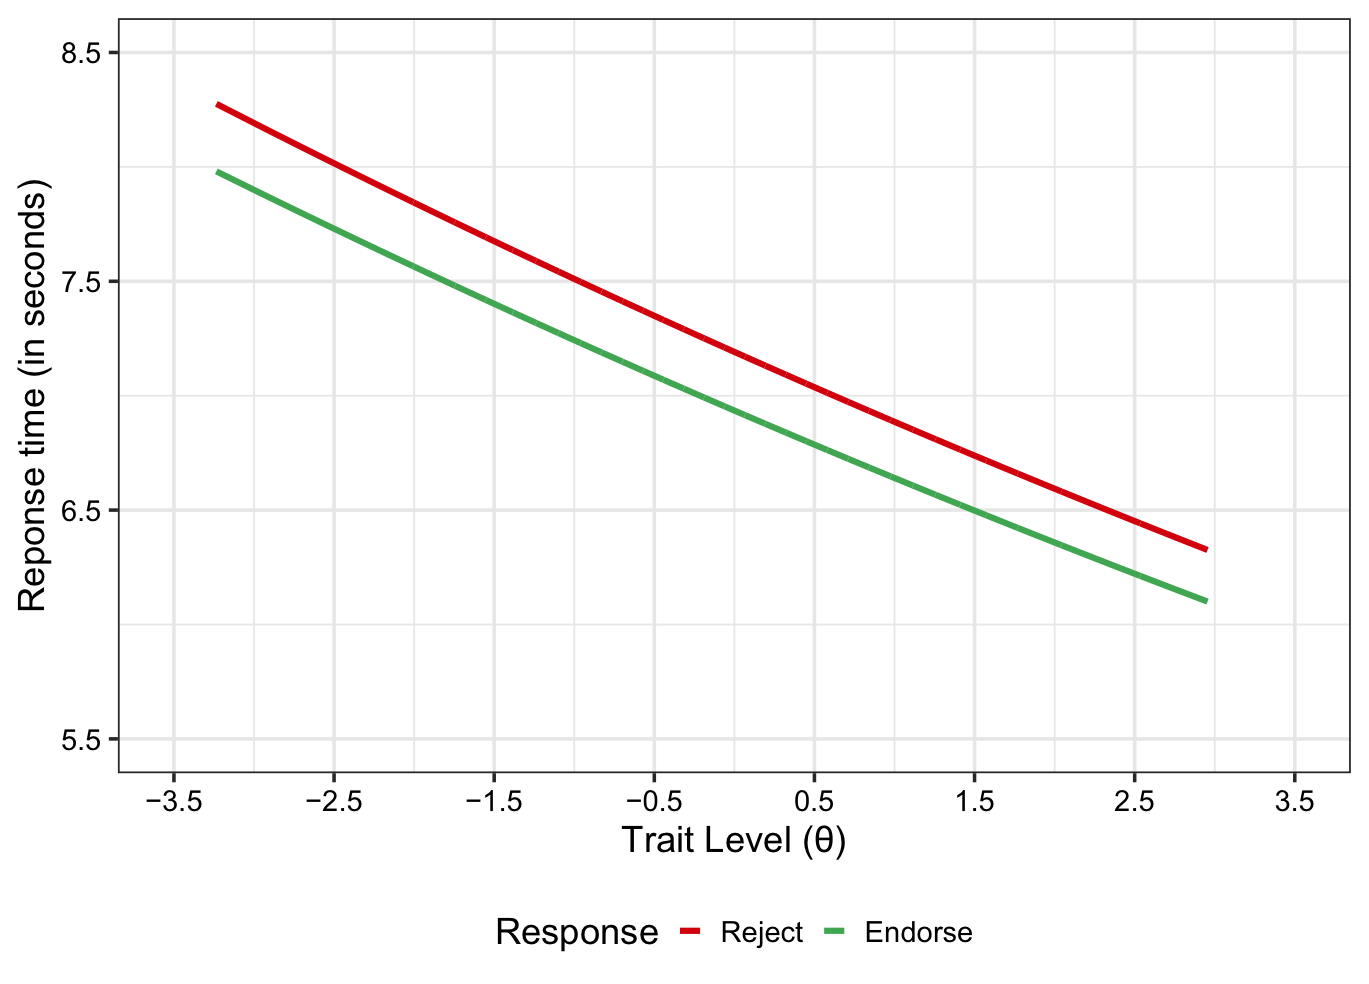
\includegraphics[keepaspectratio]{images/Poster-Figure-1-01.png}}

}

\caption{\label{fig-Figure1}From Model A3, predicted response times
according to respondent's trait level and whether the respondent
rejected the item (red) or endorsed it (green).}

\end{figure}%

\begin{figure}

\centering{

\pandocbounded{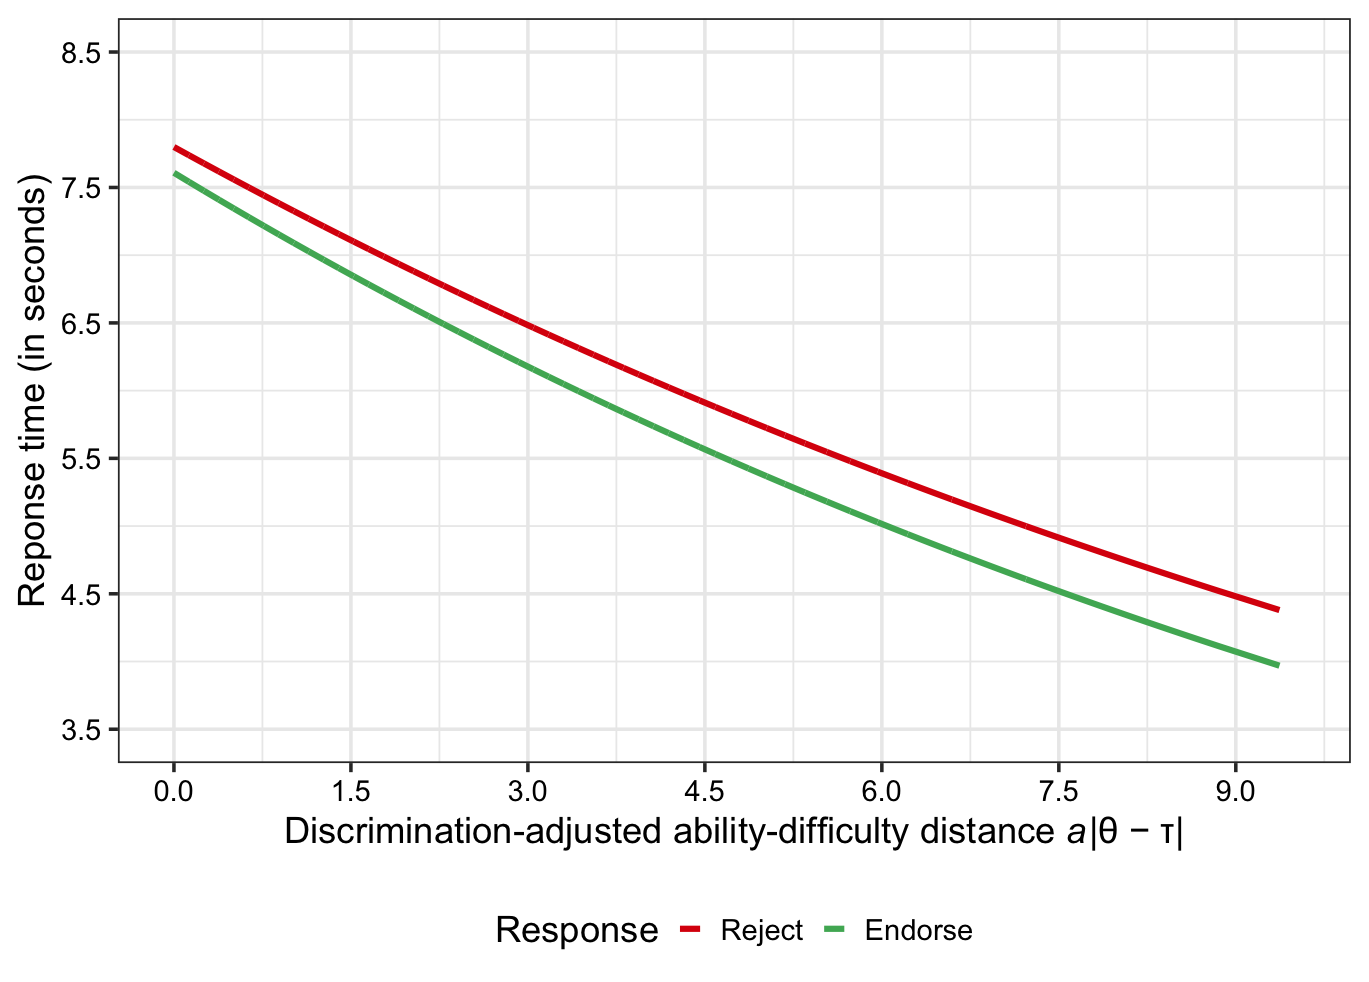
\includegraphics[keepaspectratio]{images/Poster-Figure-2-01.png}}

}

\caption{\label{fig-Figure2}From Model B3, predicted response times
according to the discrimination-adjusted distance between the
respondent's trait level and the item's neutral threshold
(``ability-difficulty distance''), by whether the respondent rejected
the item (red) or endorsed it (green).}

\end{figure}%

\section*{Appendix}\label{appendix}
\addcontentsline{toc}{section}{Appendix}

\subsection*{Appendix 1. MACH-IV Scale
Items}\label{appendix-1.-mach-iv-scale-items}
\addcontentsline{toc}{subsection}{Appendix 1. MACH-IV Scale Items}

\begin{longtable}[]{@{}
  >{\raggedright\arraybackslash}p{(\linewidth - 2\tabcolsep) * \real{0.2639}}
  >{\raggedright\arraybackslash}p{(\linewidth - 2\tabcolsep) * \real{0.7361}}@{}}
\toprule\noalign{}
\endhead
\bottomrule\noalign{}
\endlastfoot
\textbf{Item} & \textbf{Prompt} \\
1 & Never tell anyone the real reason you did something unless it is
useful to do so. \\
2 & The best way to handle people is to tell them what they want to
hear. \\
3R & One should take action only when sure it is morally right. \\
4R & Most people are basically good and kind. \\
5 & It is safest to assume that all people have a vicious streak and it
will come out when they are given a chance. \\
6R & Honesty is the best policy in all cases. \\
7R & There is no excuse for lying to someone else. \\
8 & Generally speaking, people won't work hard unless they're forced to
do so. \\
9R & All in all, it is better to be humble and honest than to be
important and dishonest. \\
10R & When you ask someone to do something for you, it is best to give
the real reasons for wanting it rather than giving reasons which carry
more weight. \\
11R & Most people who get ahead in the world lead clean, moral lives. \\
12 & Anyone who completely trusts anyone else is asking for trouble. \\
13 & The biggest difference between most criminals and other people is
that the criminals are stupid enough to get caught. \\
14R & Most people are brave. \\
15 & It is wise to flatter important people. \\
16R & It is possible to be good in all respects. \\
17 & P.T. Barnum was wrong when he said that there's a sucker born every
minute. \\
18 & It is hard to get ahead without cutting corners here and there. \\
19* & People suffering from incurable diseases should have the choice of
being put painlessly to death. \\
20 & Most people forget more easily the death of their parents than the
loss of their property. \\
\end{longtable}

\emph{Note.} Items ending in * were dropped due to insufficient factor
loadings. Reprinted from Christie and Geis (1970).

\subsection*{Appendix 2. List of Models
Used}\label{appendix-2.-list-of-models-used}
\addcontentsline{toc}{subsection}{Appendix 2. List of Models Used}

Null Model (Model 0):

\[
\ln{(t_{ij})} = \mu + \nu_j + \beta_i + \epsilon_{ij}
\]

Model A1:

\[
\ln{(t_{ij})} = \mu + \nu_j + \beta_i + \gamma_1 E_{ij} + \epsilon_{ij}
\]

Model A2:

\[
\ln{(t_{ij})} = \mu + \nu_j + \beta_i + \gamma_1 E_{ij} + \gamma_2\tau_{i,N} + \gamma_3 \theta_j + \epsilon_{ij}
\]

Model A3:

\[
\ln{(t_{ij})} = \mu + \nu_j + \beta_i + \gamma_1 E_{ij} + \gamma_2\tau_{i,N} + \gamma_3 \theta_j + \gamma_{13} E_{ij} \theta_j+ \epsilon_{ij}
\]

Model B1:

\begin{align}
\ln{(t_{ij})} &= \mu + \nu_j + \beta_i + \gamma_4 a_i |\theta_j - \tau_{i,N}|+ \epsilon_{ij} \\
&=\mu + \nu_j +\beta_i +\gamma_4\delta_{ij}+\epsilon_{ij}
\end{align}

Model B2:

\begin{align}
\ln{(t_{ij})} &= \mu + \nu_j + \beta_i + \gamma_4 a_i |\theta_j - \tau_{i,N}|+ \gamma_1E_{ij}+\epsilon_{ij} \\
&=\mu + \nu_j +\beta_i +\gamma_4\delta_{ij}+\gamma_1 E_{ij}+\epsilon_{ij}
\end{align}

Model B3:

\begin{align}
\ln{(t_{ij})} &= \mu + \nu_j + \beta_i + \gamma_4 a_i |\theta_j - \tau_{i,N}|+ \gamma_1E_{ij}+\gamma_{14}E_{ij}a_i|\theta_j-\tau_{i,N}|+\epsilon_{ij} \\
&=\mu + \nu_j +\beta_i +\gamma_4\delta_{ij}+\gamma_1 E_{ij}+\gamma_{14}E_{ij}\delta_{ij}+\epsilon_{ij}
\end{align}


\nocite{*}



\end{document}
